\documentclass[11pt]{article}
\usepackage[utf8]{inputenc}
\usepackage[spanish,es-tabla,es-nodecimaldot]{babel}

% Paquetess

\usepackage{amsmath}
\usepackage{amsthm}
\usepackage{amsfonts}
\usepackage{amssymb}
\usepackage{makeidx}
\usepackage{graphicx}
\usepackage{lmodern}
\usepackage[dvipsnames]{xcolor} 
\usepackage{fancyhdr}
\usepackage{geometry}
\usepackage{lastpage}		
\usepackage{array}			 % Para fjar tamaño de columnas
\usepackage{tikz}
\usepackage{subcaption}
\usepackage{caption}
\usepackage{pgfplots} % Para controlar la perspectiva
\RequirePackage{siunitx}
\usepackage{extramarks} % Para poder usar firstleftmarks
\usepackage[version=4]{mhchem} % Para poder usar formulas de reacciones nucleares
\usepackage{xcolor}
\RequirePackage[most]{tcolorbox}
\usepackage{enumitem}
\usepackage{physics}
%\usepackage{background}
\usepackage{eso-pic} % Para insertar imágenes de fondo específicas
\usepackage[absolute,overlay]{textpos} % Paquete para colocar elementos en posiciones absolutas
\usepackage{wrapfig}



\newtcolorbox{mybox}{colback=black!5!white,
	colframe=black!75!black}

\newtcolorbox{Anotacion}{colback=red!5!white,
	colframe=red!75!red}


%##############################################################################
%######### Ponemos el decimal con . ###########################################
%##############################################################################

\sisetup{output-decimal-marker={.},
	% exponentes ------------------------
	exponent-mode=threshold,
	exponent-thresholds=-3:2, % non usar exponentes 10^{-2,-1, 0, 1}
	% redondear -------------------------
	% round-mode=figures, % cifras sig
	% round-mode=places, % cantos decimales
	round-mode=uncertainty, % cifras sig da incerteza (necesario usar erro)
	round-precision=2,
	uncertainty-mode = separate,
	print-unity-mantissa=false,
	% unidades --------------------------
	inter-unit-product = \ensuremath{{}\cdot{}}, % separacion entre unidades
	% per-mode=power-positive-first, % so furrula con metodo interpretado puro
	inline-per-mode=single-symbol,
	display-per-mode=fraction,
}

%##############################################################################
%######### Para codigo python #################################################
%##############################################################################

\definecolor{codegreen}{rgb}{0,0.6,0}
\definecolor{codegray}{rgb}{0.5,0.5,0.5}
\definecolor{codepurple}{rgb}{0.58,0,0.82}

\usepackage{listings}


%\lstdefinestyle{mystyle}{	backgroundcolor=\color{backcolour},   	commentstyle=\color{codegreen},	keywordstyle=\color{magenta},	numberstyle=\tiny\color{codegray},	stringstyle=\color{codepurple},	basicstyle=\ttfamily\footnotesize,	breakatwhitespace=false,         	breaklines=true,                 	captionpos=b,                    	keepspaces=true,                 	numbers=left,                    	numbersep=5pt,                  	showspaces=false,                	showstringspaces=false,	showtabs=false,                  	tabsize=2}

%\lstset{style=mystyle}
%\usepackage{background}     % Para manejar el fondo


%##############################################################################
%######### Tipo de fuente #################################################
%##############################################################################

\usepackage{newtxtext,newtxmath} % Cambia la fuente (pero mola)
%\usepackage{kpfonts}

%\usepackage{helvet} 
%\renewcommand{\familydefault}{\sfdefault}.

%\usepackage{fontspec} % Paquete necesario para seleccionar fuentes
%\setmainfont{Verdana} % Cambia la fuente principal a Verdana


%##############################################################################
%######### Geometría #################################################
%##############################################################################

\geometry{a4paper, total={152mm,237mm}, left=31mm, top=30mm}



%##############################################################################
%######### Formatos capítulo #################################################
%##############################################################################

%\usepackage[lmodern]{quotchap}
%\usepackage[options]{fncychap}
% Configuración de la imagen de fondo solo para la portada



%##############################################################################
%######### Hiperreferenias #################################################
%##############################################################################


\usepackage[colorlinks=true, linkcolor=RoyalBlue, citecolor=ForestGreen, urlcolor=BrickRed]{hyperref} % Crea las
\usepackage[nameinlink]{cleveref}
\crefname{figure}{Fig.}{Figs.}

%##############################################################################
%######### Formato de pagina #################################################
%##############################################################################

\pagestyle{fancy}
\fancyhf{} % Limpia encabezados y pies
\fancyhead[L]{\small \textbf{Respuestas Nuclear}}    % Encabezado izquierdo
\fancyhead[R]{\small \textbf{Daniel Vázquez, Laura Quintáns}}     % Encabezado derecho
\fancyfoot[C]{\thepage}      % Pie de página centrado con el número de página
\renewcommand{\headrulewidth}{0.4pt}  % Grosor de la línea del encabezado
\renewcommand{\footrulewidth}{0pt}    % Sin línea en el pie



%##############################################################################
%#########  Modificar caption #################################################
%##############################################################################

\usepackage[font=small, justification=centering]{caption}  % Configura las captions



%##############################################################################
%######### Comandos propios #################################################
%##############################################################################


\newcommand{\parentesis}[1]{\left( #1  \right)}
\newcommand{\parciales}[2]{\frac{\partial #1}{\partial #2}}
\newcommand{\pparciales}[2]{\parentesis{\parciales{#1}{#2}}}
\newcommand{\ccorchetes}[1]{\left[ #1  \right]}
\newcommand{\D}{\mathrm{d}}
\newcommand{\derivadas}[2]{\frac{\D #1}{\D #2}}

\newcommand{\tquad}{\quad \quad \quad}
%\newcommand{\vnabla}{\vec{\nabla}}

\newcommand{\Ocal}{\mathcal{O}}
\newcommand{\Jcal}{\mathcal{J}}
\newcommand{\Mcal}{\mathcal{M}}
\newcommand{\Fcal}{\mathcal{F}}
\newcommand{\Hcal}{\mathcal{H}}
\newcommand{\Ecal}{\mathcal{E}}
\newcommand{\Ncal}{\mathcal{N}}

\newcommand{\cmm}{\text{cm}^{-1}}
\newcommand{\fcc}{\textit{fcc}}
\newcommand{\bcc}{\textit{bcc}}
\renewcommand{\sc}{\textit{sc}}
\newcommand{\hcp}{\textit{hcp}}


\newcommand{\PZB}{\text{{\tiny PZB}}}
\newcommand{\gap}{\text{{\tiny gap}}}
\newcommand{\SZB}{\text{{\tiny SZB}}}
\newcommand{\inicial}{\text{{\tiny inicial}}}
\newcommand{\final}{\text{{\tiny final}}}
\newcommand{\atomico}{\text{{\tiny atómico}}}

\newcommand{\arctanh}{\text{{arctanh}}}



\newcommand{\Namas}{\text{Na}^+}
\newcommand{\Clmenos}{\text{Cl}^-}

\newcommand{\cm}{\text{cm}}
\newcommand{\eV}{\text{eV}}

\newcommand{\arr}{\text{arr}}
\newcommand{\diff}{\text{diff}}

\newcommand{\er}{$^{\text{er}}$}
\newcommand{\cte}{\text{cte}}


% Comandos vectoriales

\newcommand{\an}{\mathbf{a}}
\newcommand{\bn}{\mathbf{b}}
\newcommand{\dn}{\mathbf{d}}
\newcommand{\fn}{\mathbf{f}}
\newcommand{\jn}{\mathbf{j}}
\newcommand{\kn}{\mathbf{k}}
\newcommand{\pn}{\mathbf{p}}
\newcommand{\qn}{\mathbf{q}}
\newcommand{\rn}{\mathbf{r}}
\newcommand{\sn}{\mathbf{s}}
\newcommand{\un}{\mathbf{u}}
\newcommand{\vn}{\mathbf{v}}
\newcommand{\xn}{\mathbf{x}}
\newcommand{\wn}{\mathbf{w}}
\newcommand{\yn}{\mathbf{y}}
\newcommand{\qndot}{\dot{\qn}}

\newcommand{\alphan}{\boldsymbol{\alpha}}
\newcommand{\sigman}{\boldsymbol{\sigma}}
\newcommand{\pin}{\boldsymbol{\pi}}
\newcommand{\rhon}{\boldsymbol{\rho}}
\newcommand{\epsilonn}{\boldsymbol{\epsilon}}
\newcommand{\omegan}{\boldsymbol{\omega}}
\newcommand{\mun}{\boldsymbol{\mu}}



\newcommand{\An}{\mathbf{A}}
\newcommand{\Bn}{\mathbf{B}}
\newcommand{\En}{\mathbf{E}}
\newcommand{\Fn}{\mathbf{F}}
\newcommand{\Jn}{\mathbf{J}}
\newcommand{\Hn}{\mathbf{H}}
\newcommand{\Gn}{\mathbf{G}}
\newcommand{\Kn}{\mathbf{K}}
\newcommand{\Ln}{\mathbf{L}}
\newcommand{\Mn}{\mathbf{M}}
\newcommand{\Pn}{\mathbf{P}}
\newcommand{\Rn}{\mathbf{R}}
\newcommand{\Sn}{\mathbf{S}}
\newcommand{\Tn}{\mathbf{T}}
\newcommand{\In}{\mathbf{1}}
\newcommand{\Encal}{\boldsymbol{\mathcal{E}}}

\newcommand{\hnn}{\hat{\mathbf{n}}}
\newcommand{\hnr}{\hat{\mathbf{r}}}
\newcommand{\hnz}{\hat{\mathbf{z}}}
\newcommand{\hnv}{\hat{\mathbf{v}}}
\newcommand{\hnx}{\hat{\mathbf{x}}}
\newcommand{\hny}{\hat{\mathbf{y}}}
\newcommand{\hnu}{\hat{\mathbf{u}}}
\newcommand{\hnR}{\hat{\mathbf{R}}}
\newcommand{\hnp}{\hat{\mathbf{p}}}
\newcommand{\hnk}{\hat{\mathbf{k}}}
\newcommand{\hni}{\hat{\mathbf{i}}}
\newcommand{\hnj}{\hat{\mathbf{j}}}
\renewcommand{\hnk}{\hat{\mathbf{k}}}


% Autor y título

%\author{Daniel Vazquez Lago}
\title{Repuestas Grupo IV Pareja VII Dispersión Compton}


\begin{document}
	
\maketitle
\tableofcontents

\setlength{\parskip}{1.5mm} % Cambia el espacio entre párrafos

\newpage


%%%%%%%%%%%%%%%%%%%%%%%%%%%%%%%%%%%%%%%%%%
%%%%%%%%%%%%%%% TEORÍA %%%%%%%%%%%%%%%%%%%% 
%%%%%%%%%%%%%%%%%%%%%%%%%%%%%%%%%%%%%%%%%%


\section{Teoría}

\subsection{¿Qué es la dispersión Compton?}

El efecto Compton es el proceso por el cual un fotón de alta energía (como un rayo gamma) interactúa de forma inelástica con un electrón (que puede considerarse libre o débilmente ligado), perdiendo parte de su energía y aumentando su longitud de onda. La energía perdida por el fotón se transfiere al electrón, que es expulsado con una energía cinética correspondiente. La relación entre el ángulo de dispersión del fotón y el cambio en su energía se describe mediante la fórmula de Compton. Este fenómeno es fundamental para entender la interacción de la radiación electromagnética con la materia y tiene implicaciones directas en espectros de detección gamma, donde se observa un continuo de Compton y se marca el borde Compton en el espectro.

\subsection{Eficiencia geométrica e intrínseca}
La eficiencia geométrica se refiere a la fracción de la radiación emitida por la fuente que llega efectivamente al detector. Dado que la fuente suele emitir isotrópicamente, la radiación se distribuye sobre una esfera cuya superficie es $4\pi d^2$ (siendo d la distancia a la fuente). Por ello, si el área activa del detector es $A$, la eficiencia geométrica se puede calcular como:

\begin{equation}
    \varepsilon_{\text{geo}} = \frac{A}{4\pi d^2} = \frac{N_{\text{llegadas}}}{N_{\text{emitidas}}}
\end{equation}
En cambio, la eficiencia intrínseca se refiere a la probabilidad de que un fotón que incide en el detector interactúe y se convierta en una señal útil (por ejemplo, depositando toda o parte de su energía de forma que se registre en el fotópico correspondiente). Esta eficiencia depende de las propiedades del material detector (su composición, grosor, etc.) y de los procesos de interacción que predominen a esa energía (como el efecto fotoeléctrico, la dispersión Compton o la producción de pares).

\begin{equation}
    \varepsilon_{\text{int}} = \frac{N_{\text{detectadas}}}{N_{\text{llegadas}}} 
\end{equation}

En otras palabras, mientras la eficiencia geométrica está determinada únicamente por la disposición y las dimensiones del sistema experimental, la eficiencia intrínseca caracteriza la capacidad del detector para "capturar" y registrar la radiación que le llega. La eficiencia total de detección es el producto de ambas:

\begin{equation}
    \varepsilon=\varepsilon_{\text{geo}} \times \varepsilon_{\text{int}}
\end{equation}

\subsection{Informacion de interés}

El detector de silicio media (rectángulo negro en la tapa superior) medía 2 cm de largo, 1 cm de ancho y x de altura (la altura está medida por edentro). \\


El detector es una caja de Yoduro de Cesio dopado con Talio con un detector de Silicio. 



%%%%%%%%%%%%%%%%%%%%%%%%%%%%%%%%%%%%%%%%%%%%%%%%%%%%%%%
%%%%%%%%%%%%%%% RESUMEN E INDICACIONES %%%%%%%%%%%%%%% 
%%%%%%%%%%%%%%%%%%%%%%%%%%%%%%%%%%%%%%%%%%%%%%%%%%%%%%%

\newpage

\section{Resumen e indicaciones}

\subsection{Adquisición de espectros [3h]}

Lo primero es adquirir los espectros de las diferentes fuentes gamma. El \textbf{espectro gamma} de una determinado núcleo nos dice cuantos fotones se emiten para una determinada longitud de onda o frecuencia. Tenemos varias fuentes en el laboratorio, y tendremos que adquirir los espectros de todas ellos. Veamos cuales son los espectroes de las fuentes, para saber que resultados podemos obtener: 

\begin{itemize}
    \item \textbf{\(^{152}\)Eu (Europio-152):} Fuente de calibración con un espectro gamma complejo que abarca desde aproximadamente 120\,keV hasta más de 1400\,keV. Se decae mediante captura electrónica y beta, y posee una vida media de alrededor de 13,5 años.
    %\begin{figure}[h!] \centering
      %  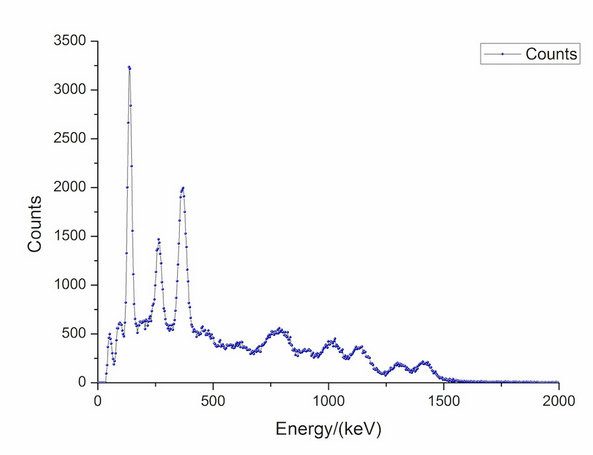
\includegraphics[width=0.5\linewidth]{152Eu.png}      
     %   \caption{Espectro gamma del 152Eu}  
    %\end{figure}
    \item \textbf{\(^{60}\)Co (Cobalto-60):} Emite dos rayos gamma de aproximadamente 1173\,keV y 1332\,keV en cascada tras una desintegración beta a \(^{60}\)Ni. Es ampliamente utilizado en aplicaciones médicas e industriales, con una vida media de aproximadamente 5,27 años.
    %\begin{figure}[h!] \centering
      %  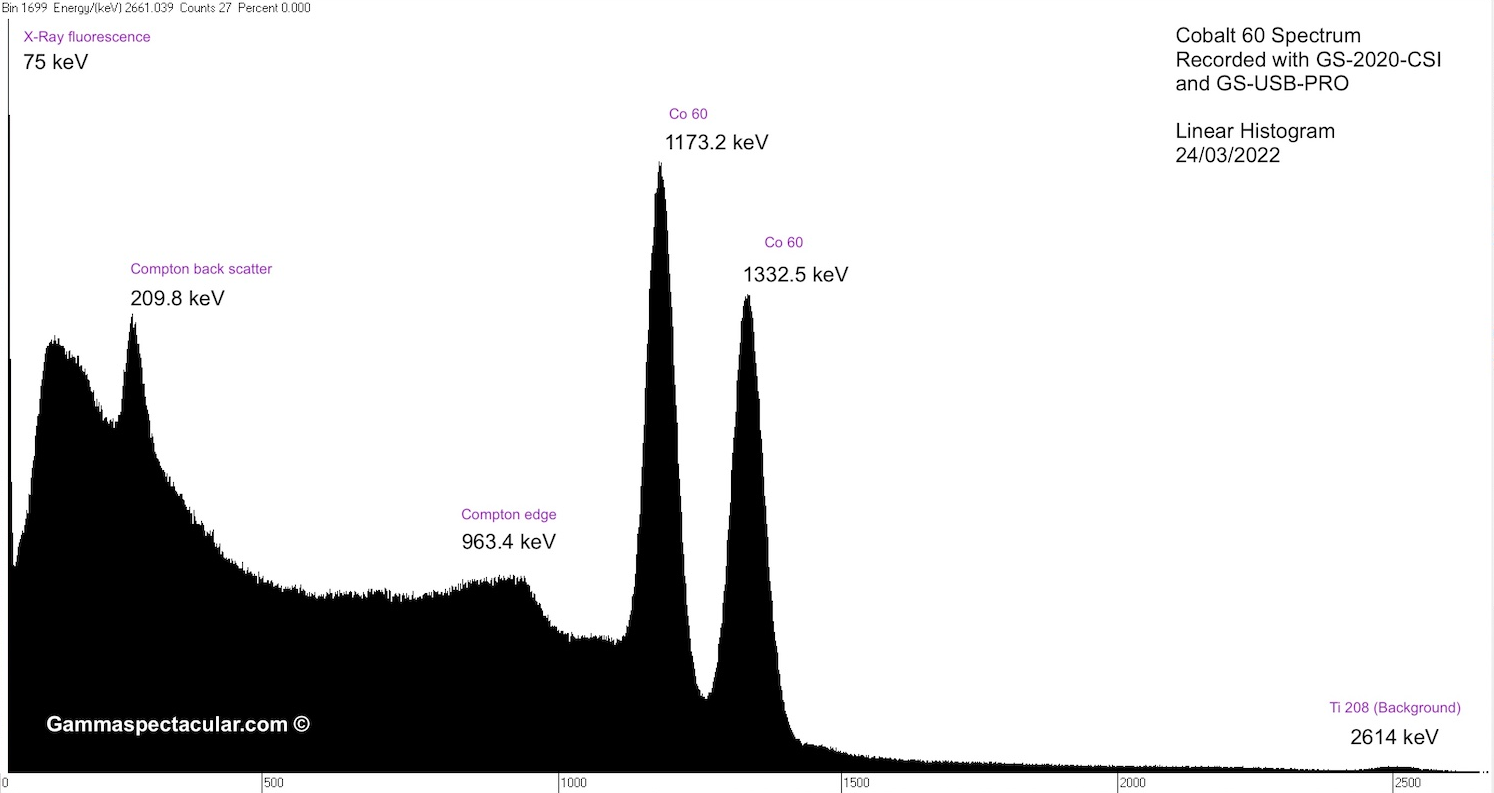
\includegraphics[width=0.5\linewidth]{60Co.png}    
     %   \caption{Espectro gamma del 60Co}      
    %\end{figure}
    \item \textbf{\(^{137}\)Cs (Cesio-137):} Emite un único rayo gamma de 661,7\,keV tras la desintegración beta y la consiguiente transición isomérica de \(^{137}\)Ba. Es una fuente habitual en estudios de calibración, con una vida media de aproximadamente 30,1 años.
    %\begin{figure}[h!] \centering
     %   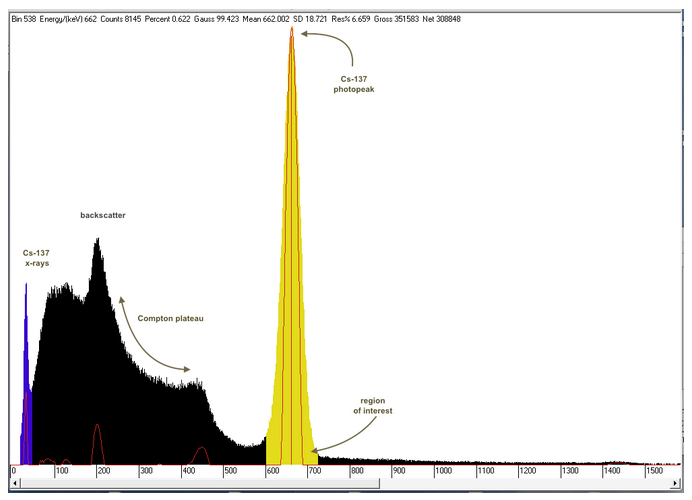
\includegraphics[width=0.5\linewidth]{137Cs.png}      
    %    \caption{Espectro gamma del 137Cs}    
   % \end{figure}
    \item \textbf{\(^{22}\)Na (Sodio-22):} Se decae mediante emisión de positrones (y en menor medida por captura electrónica), generando dos rayos gamma de 511\,keV por aniquilación y otro de 1274,5\,keV. Su vida media es de unos 2,6 años. 
 %   \begin{figure}[h!] \centering
  %      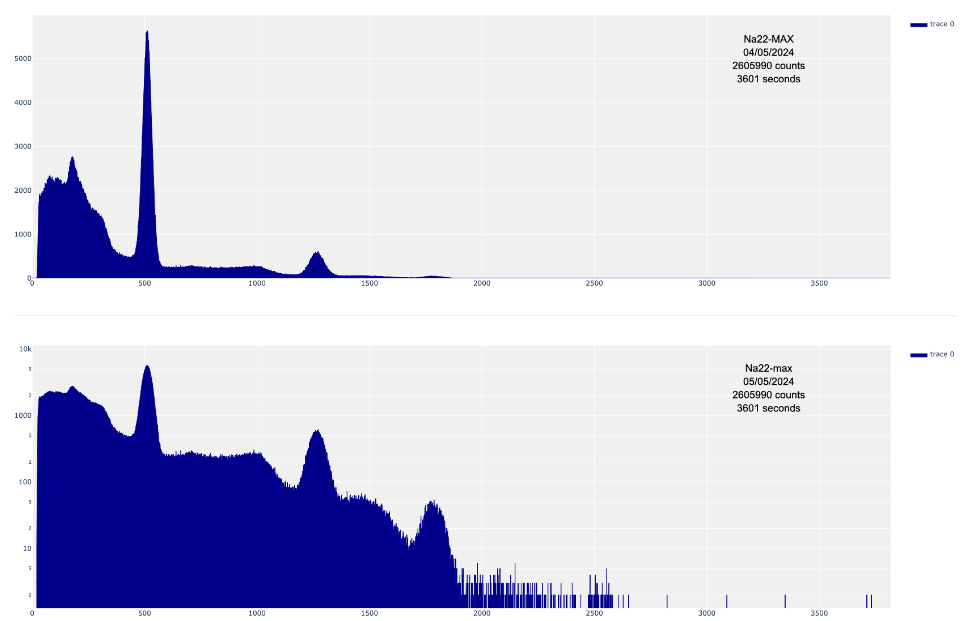
\includegraphics[width=0.6\linewidth]{22Na.png}    
  %      \caption{Espectro gamma del 22Na}      
  %  \end{figure}
    \item \textbf{\(^{207}\)Bi (Bismuto-207):} Emite varios rayos gamma (destacando líneas alrededor de 570\,keV y 1063\,keV) tras la captura electrónica. Es útil para calibraciones y estudios espectrométricos, con una vida media aproximada de 31,55 años.
\end{itemize}
Es muy \textcolor{BrickRed}{importante determinar la geometría del sistema: distancia engtre fuente y entrada del detector} y también es \textcolor{Blue}{importante colocar las fuentes a una distancia fija y bien centradas}.


\subsection{Calibración del detector [30min]}

Ahora tenemos que calibrar el aparato, con lo que podremos determinar las energías a las que se producen las diferentes características del fondo ambiental. Hacer una calibración energética de cada detector utilizando la información obtenida en el análisis significa establecer una relación precisa entre la señal medida (por ejemplo, el número de canal o la amplitud de la señal) y la energía real de las radiaciones detectadas. Para ello, se utilizan datos experimentales—como picos conocidos o líneas espectrales de fuentes con energías establecidas—que permiten construir una función (usualmente lineal o polinómica) que transforma la escala de canales en una escala de energías.

Primero tenemos que definir qué es la \textbf{ganancia}. La ganancia del sistema es un parámetro que indica cómo se amplifica la señal de luz detectada. En esencia, define la relación entre la señal eléctrica (por ejemplo, en voltios o en un número de canales) y la energía real de la radiación incidente. Si la ganancia aumenta, una misma cantidad de energía se traduce en una señal más intensa, y si disminuye, la señal es más débil. Esta ganancia puede variar entre diferentes mediciones debido a fluctuaciones en el sistema o a cambios en sus condiciones operativas.

Cuando se adquieren espectros, estas variaciones en la ganancia pueden desplazar la posición de los picos en los canales. Por ello, si se intenta restar el espectro del fondo ambiental a los espectros de las fuentes radiactivas antes de calibrarlos en energía, la diferencia en la asignación de canales entre las mediciones hará que la sustracción no sea precisa y que queden restos de fondo o se eliminen partes útiles de la señal.

Sin embargo, si se realiza una calibración en energía primero, se corrige esa variación de ganancia. La calibración ajusta la escala de los espectros para que los picos correspondan a las energías correctas, independientemente de las fluctuaciones en la ganancia. Una vez calibrados, al restar el espectro del fondo (también calibrado) del espectro de la fuente, se elimina de forma precisa la contribución ambiental, ya que ambas mediciones están en la misma escala de energía.


\subsection{Dependencia espectros y distancia detector-fuente [1h]}

Para una fuelte de alta actividad y que presente un fotopico bien diferenciado, comprobamos cual es la dependencia de la llegada de radiación al fotopico para diferentes distancias. \textcolor{Blue}{Mínimo 8 distancias con la mayor precisión posible, fuente bien centrada respecto a la proyección de la entrada del detector.} tendremos que hacer, posteriormente, análisis y aproximaciones de la eficiencia energética con la distancia bajo diferentes modelos.

\subsection{Dependencia anchura y energia del fotopico [30min]}

Sobre los espectros observados se puede estudiar la anchura de los fotópicos observados, mediante algún parámetro estadístico significativo como la anchura total a media altura. La FWHM (Full Width at Half Maximum) es la anchura total de un pico en un espectro, medida a la mitad de su altura máxima. Es decir, se define como la diferencia entre los dos valores de la variable (por ejemplo, energía) en los cuales la intensidad del pico alcanza el 50\% de su valor máximo. Este parámetro es fundamental para cuantificar la resolución de un sistema de detección: una FWHM pequeña indica una mejor resolución y menor dispersión en la respuesta del detector.

\subsection{Eficiencia: determinación y dependencia con la energía [1h]}

No toda la radiación gamma emitida produce una cuenta en la energía que le corresponde. Parte de la radiación emitida no llega nunca al detector (recordad que la emisión es isótropa, se emite en todas las direcciones uniformemente) y parte de la que llega al detector no es detectada y lo atraviesa o no contribuye al fotopico al no depositarse completamente su energía en el material activo del detector. Con todo, tenemos que utilizar la información dispnible en los apartados anteriores para intentar comprobar dos cosas:

\begin{enumerate}
    \item Si las formulaciones sobre la eficiencia geométrica son correctas y si realmente se obtiene un conteo en el fotopico de acuerdo con la dependencia cona la distancia esperada.
    \item Si, una vez descontada la eficiencia geométrica, podemos determinar la eficiencia intrínseca que corresponde a cada fotopico y de ahí derivar cual es la dependencia de la eficiencia intrínseca con la energía del fotopico.
\end{enumerate}

\subsection{Montaje y prueba para medir dispersión Compton [1h]}

Para poder determinar propiedades de la dispersión Compton necesitamos montar un sistema en el que midamos el efecto al incidir un haz colimado entrante en un centro dispersor, una pequeña pieza de metacrilato. Usaremos una fuente de muy alta actividad. La colmación se realizará a través de bloques de plomo, con la que definri una dirección única para la radiación emitida que incida sobre el centro dispersor. COlocaremos el detector a diferentes ángulos y a distancia fija del centro dispersor para medir el espectro dispersado por sus electrones mediante la interacción Compton. 

\subsection{Relación energía, ángulo y sección eficaz [5h]}

Pasaremos a la medida sistemática de los espectros de energía para diferentes ángulos entre el centro dispersor y el detector (con respecto a la línea determinada por la incidencia de la radiación gamma sobre el centro dispersor). Cada meida se realiza con y sin dispersor, para pdoer restar todas las dispersiones de la radiación producidas porla interacción de la radiación de la fuente con el resto de materia de vuestro dispositivo. Así, al restar ambos espectros, sólo se observarán las dispersiones producidas por el centro dispersor. Por simplicidad, \textcolor{Blue}{os recomdamos medir la misma cantidad de tiempo con y sin centro dispersor en cada uno de los ángulos}.



\newpage

%%%%%%%%%%%%%%%%%%%%%%%%%%%%%%%%%%%%%%%%%%
%%%%%%%%%%%%%%% PREGUNTAS %%%%%%%%%%%%%%%% 
%%%%%%%%%%%%%%%%%%%%%%%%%%%%%%%%%%%%%%%%%%


\section{Preguntas}


\subsection{Adquisición de los espectros}
\begin{enumerate}[label=\alph*)]
    \item ¿Cuánto tiempo tengo que medir para determinar razonablemente las características de los espectros?
    \item ¿Cuáles son estas características básicas? ¿Observo los fotópicos esperados? ¿Se pueden observar los continuos Compton, el borde Compton, picos de retrodispersión? ¿Qué otros efectos observas?
    \item ¿Cómo es el espectro del fondo ambiental? ¿Qué fuentes de radiación dominan en ese fondo? ¿Puedes identificar algún fotópico?
    \item ¿Cómo obtienes el número total de partículas emitidas de un tipo determinado por la fuente radiactiva? ¿Sabrías definir los conceptos de coeficiente de ramificación y de intensidad relativa? ¿Puede ser la intensidad relativa de emisión superior al 100\%? ¿Y la suma de las intensidades relativas? Calcula en detalle el número de radiaciones de cada energía que deberían emitir las fuentes.
\end{enumerate}

\subsection{Calibración de los detectores}
\begin{itemize}
    \item ¿Observas desviaciones en la posición de algunos picos respecto a la recta de calibración? En caso de observarse, ¿para qué picos y por qué posibles razones aparecen estas desviaciones?
    \item ¿Puedes deducir de tus datos una variación de la recta de calibración con el tiempo transcurrido o con el cambio de temperatura? ¿Qué tipo de variación observas?
\end{itemize}

\subsection{Determinación de la dependencia con la distancia entre fuente y detector}
\begin{itemize}
    \item ¿Observas algún cambio en la energía asociada al fotópico con la distancia de la fuente al detector? ¿Cómo interpretas este resultado?
    \item ¿Cuál crees que es, a priori, la forma funcional que tendrá la tasa de llegada de radiación en el fotópico con la variación de la distancia? ¿Crees que será la misma para cada fotópico?
\end{itemize}

\subsection{Estudio de la dependencia de la anchura de los fotópicos con la energía}
\begin{itemize}
    \item ¿Son todos los fotópicos de la misma anchura o se observa alguna tendencia?
    \item ¿Puedes dar un valor aproximado de la FWHM para un fotópico a baja energía y otro a alta energía? Si definimos la resolución \( R = \frac{\mathrm{FWHM}}{\mathrm{energia}} \), ¿puedes dar valores de la resolución a esas energías?
    \item Podéis encontrar fotópicos de diferentes fuentes que se encuentran a energías similares. ¿Tienen la misma anchura estos fotópicos o dependen de la fuente?
    \item ¿Podéis localizar algún fotópico que, ya en un análisis preliminar, no cumpla con la dependencia con la energía que parecen seguir el resto de fotópicos? En caso de observarlo, intentad descubrir la razón en función de sus propiedades.
\end{itemize}

\subsection{Determinación de la eficiencia geométrica e intrínseca de detección}
\begin{itemize}
    \item ¿A qué potencia de la distancia entre fuente y detector se espera que caiga la eficiencia geométrica? ¿Puedes imaginar que efectos modifiquen este comportamiento?
    \item La eficiencia intrínseca de cada fotópico cambia por la energía… ¿puedes imaginar qué procesos en cada rango de energía producen la variación de la eficiencia?
    \item ¿Puedes dar un valor aproximado de la eficiencia intrínseca para un fotópico a baja energía y otro a alta energía? ¿De qué crees que depende la eficiencia intrínseca del detector a una energía determinada?
\end{itemize}

\subsection{Montaje y prueba de un sistema para medir la dispersión Compton}
\begin{itemize}
    \item La apertura del colimador delimita la cantidad de radiación gamma que le llega al centro dispersor. ¿Podéis calcular cuál es la cantidad de gammas que llega por cm\(^2\) del centro dispersor a partir de la actividad de la fuente y de la distancia fuente–centro dispersor?
    \item El montaje requiere que se puedan medir a diferentes ángulos a un lado y otro respecto al eje central a cero grados sin dispersión. ¿Es simétrica la dispersión Compton? ¿Por qué creéis que es necesario medir a ambos lados del eje central?
    \item Para determinar las secciones eficaces de dispersión es necesario medir con la mayor precisión posible las distancias tanto entre el centro de la fuente radiactiva y el centro del dispersor como entre el centro del dispersor a la ventana de entrada del detector. ¿Cómo os parece que debería ser esta última distancia, lo más pequeña posible o lo mayor posible? Discutid los pros y contras de cada posición.
\end{itemize}

\subsection{Medida de la relación energía-ángulo y de la sección eficaz de dispersión}
\begin{itemize}
    \item El centro dispersor es un bloque de metacrilato cilíndrico. ¿Puedes calcular el número de centros dispersores (electrones) que tiene cada cm\(^3\) de metacrilato? Asegúrate de usar la fórmula estequiométrica correcta para el metacrilato.
    \item Resta los espectros con y sin centro dispersor. ¿Encuentras canales de energía para los que se tienen valores negativos en el espectro resta? ¿Cómo se interpreta esto? ¿Qué valores promedio esperas obtener en una región amplia energética en la que no hay dispersión Compton del centro dispersor? ¿Y qué valores máximos esperas tener para la dispersión alrededor de esa media en los bines individuales?
    \item Haz un cálculo rápido para cada ángulo para determinar en qué energía debería aparecer el exceso de cuentas asociado a la dispersión Compton. ¿Cuál es la dispersión en energía de la región en la que en realidad ves un exceso de cuentas? ¿Puede explicarse esa dispersión por la geometría de tu sistema de detección?
    \item Finalmente, derivad la sección eficaz de dispersión de forma aproximada.
\end{itemize}

%%%%%%%%%%%%%%%%%%%%%%%%%%%%%%%%%%%%%%%%%%%%
%%%%%%%%%%%%%%% RESPUESTAS %%%%%%%%%%%%%%%%% 
%%%%%%%%%%%%%%%%%%%%%%%%%%%%%%%%%%%%%%%%%%%%

\newpage

\section{Respuestas}


\subsection{Adquisición de los espectros}
\begin{enumerate}[label=\alph*)]
    \item El tiempo para obtener razonablemente las características las fuentes de los espectros dependerán de la actividad, de la precisión del aparato y de la incertidumbre estadística máxima que queramos. Dado que la incertidumbre para el contaje suele venir dada por $\sqrt{N}$ donde $N$ es el número de medidas. Consecuentemente, el error relativo es $1/\sqrt{N}$. Si quisieramos por ejemplo, para un fotopico un error del $x\%$ tendríamos que:
    \begin{equation}
        N = \frac{100^2}{x^2}
    \end{equation}
    Por ejemplo para $5\%$ tendríamos $N=400$, si quisieramos $2\%$ necesitaríamos $N=2500$ y si $1\%$ tendríamos $N=10000$. El tiempo de medida dependerá entocnes de cuanto tarde en llegar a este número de cuentas la fuente gamma. Veamos para cada fuente:

    \begin{itemize}
        \item El Bismuto 207 nesitamos 800 segundos de tiempo vivo, ya que así obtuvimos una incertidumbre en los picos de 1.44,2.97,1.18 (en porcetntaje); en los canales 2167, 4000.20, 768.85 con energías 570, 1168, 175. Lo colocamos a 7.2 cm del detector. 
        \item El Sodio 20  necsitamos 832 segundos de tiempo vivo, ya que así obtuvimos una incertidumbre del 1.01\% y el 3.21\% en los canales 1944.43 y 4754.54 con energías 512 y 1264. Lo colocamos a 7 cm.
        \item El Cobalto 60 necesitamos x segundos de tiempo vivo, ya que así obtuvimos una incertidumbre del 3.8\% y 3.95\% para los canales 4392 y 4937 con energías 1173 y 1332. 
    \end{itemize}




    \item Existen las siguientes características básicas en un espectro gamma:
    \begin{itemize}
        \item \textbf{Fotópico:} Pico principal que corresponde a la deposición completa de la energía del fotón en el detector. Su posición y anchura son fundamentales para la calibración energética.
        \item \textbf{Continuo Compton:} Región ancha del espectro originada por eventos en los que el fotón deposita sólo una parte de su energía mediante dispersión Compton.
        \item \textbf{Borde Compton:} Límite superior del continuo Compton, correspondiente a la máxima energía transferible en un único evento de dispersión Compton.
        \item \textbf{Pico de retrodispersión:} Pico adicional, en ocasiones presente, que resulta de fotones dispersados en el entorno y que regresan al detector con una energía reducida.
        \item \textbf{Fondo ambiental:} Señal de fondo debida a radiación ambiental o interacciones secundarias, cuya caracterización es esencial para aislar la señal procedente de la fuente.
    \end{itemize}
    \textcolor{BrickRed}{Falta por decir si medimos los fotopicos esperados, si se pueden observar los continuos de Compoton, el borde Compoton, los picos de retrodispersión y si hay otros efectos (fondo ambiental).}
    \item El espectro de fondo ambiental debe tener la siguiente forma:
    \begin{figure}[h!] \centering
        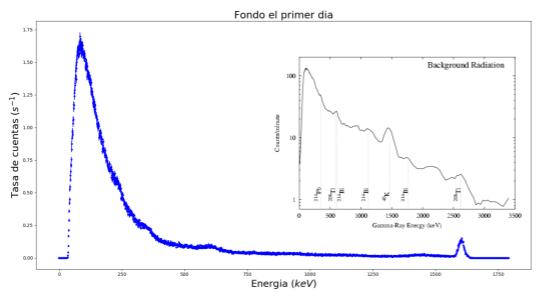
\includegraphics[width=0.6\linewidth]{Espectro_Fondo.png}
        \caption{Espectro gamma de fondo. Foto tomada de memoria de Alejandro Doval Casas.}      
    \end{figure}

    Como podemos ver hay 3 fotopicos, a las energías. En general el espectro del fondo ambiental viene dado por la radiación cósmica y la radiación terrestre. La radiación terrestre depende principalmente de la desintegración natural de algunos núcleos presentes en la corteza terrestre (por ejemplo, el Potasio-40, con su fotópico característico alrededor de 1460 keV, y los descendientes del Uranio y del Torio).\textcolor{BrickRed}{Tenemos que poner nuestro fondo ambiental, y hablar más de los fotopicos y de su identificación.}
    \item El \textbf{número total de partículas emitidas} de un tipo determinado por la fuente radioactiva lo obtenemos a través de la \textit{actividad} $A(t)$ y del \textit{braching ratio} $B$. La actividad nos da el número de eventos radioactivos de la muestra
    \begin{equation}
        A(t) = A_0 e^{-\lambda t}
    \end{equation}
    donde $A_0$ era la actividad en el instante $t=0$. Si conocieramos esta actividad, podríamos co nocer la actividad en cualquier momento. Sin embargo la actividad puede ocurrir por diferentes canales, y por tanto \textit{no toda la actividad corresponden a partículas emitidas}. Si $B_\gamma$ es la tasa de la actividad que emite fotones, entonces el número de partículas de interés emitidas (fotones) será, para un instante $t$:

    \begin{equation}
        N_{\text{emitidas}} (t) = B_\gamma A(t)
    \end{equation}
    El \textbf{coeficiente de ramificación} es precisamente lo que hemos definido como braching ratio, i.e., es la probabilidad de que una desintegración radiactiva se realice a través de una vía o canal específico. La \textbf{intensidad relativa} por otro lado es una medida experimental que representa la proporción de la radiación (o de las partículas) emitida con una energía determinada respecto al total de la radiación detectada. Por definición ni la intensidad relativa ni la suma de intensidades relativas puede ser mayor al $100\%$ de la intensidad total. Experimentalmente podría suceder si hay fallos en los detectores. \textcolor{BrickRed}{Tenemos que calcular el número de radiaciones de cada energía que deberían emitir las fuentes.}
\end{enumerate}

\subsection{Calibración de los detectores}

\begin{enumerate}[label=\alph*)]
    \item Esto puede traducirse en un desplazamiento, generalmente de carácter casi lineal, de los fotópicos respecto a la calibración establecida inicialmente. Dicho desplazamiento podría variar según la energía, ya que la respuesta del detector puede no ser perfectamente lineal en todo el rango energético. \textcolor{BrickRed}{Hay que decir sí observamos algunas desviaciones respecto la recta de calibración de algunos picos.} 
    
    Algunas de las posbiles razones son: respuesta del detector, que en ciertos rangos puede no ser estrictamente lineal, provocando que algunos picos se desvíen de la tendencia esperada. Además, las fluctuaciones en la ganancia del sistema y la resolución limitada del detector contribuyen a que los picos se desplazen o se ensanchen, dificultando la determinación exacta de sus energías. Por otro lado, la presencia de ruido, el fondo ambiental y el solapamiento de picos con energías cercanas también pueden alterar la posición precisa de los picos de calibración. Estos factores, en conjunto, generan las desviaciones observadas en la recta de calibración para nuestras fuentes. \textcolor{BrickRed}{Verificar si estas razones son correctas.}
    \item  \textcolor{BrickRed}{Es de esperar una variación lineal o exponencial con el tiempo, aunque hay que verificar los datos.}
\end{enumerate}

\subsection{Determinación de la dependencia con la distancia entre fuente y detector}

\begin{enumerate}[label=\alph*)]
    \item En condiciones ideales no se debería observar un cambio en la energía asociada al fotópico con la distancia de la fuente al detector. La energía de los fotones gamma emitidos por la fuente es una propiedad intrínseca de la transición nuclear correspondiente y no depende de la distancia que recorran hasta el detector. Sin embargo puede ocurrir que no lo sea debido a dispersión con el aire, efectos geométricos (alineación), efectos de ganancia del detector (en función del flujo de detectores cambie) y efectos térmicos. \textcolor{BrickRed}{Aún falta la interpretación.}
    \item Se espera que caiga como $1/d^2$ siendo $d$ la distancia entre la fuente y el detector. Debería ser igual para cada fotopico, con una caida de $1/d^2$. Sin embargo existen ciertos fenómenos que podrían hacer que sean diferentes: 
    \begin{itemize}
        \item Eficiencia intrínseca del detector: La probabilidad de detección de un fotón de una determinada energía depende de los procesos de interacción en el detector (fotoeléctrico, Compton, producción de pares). La eficiencia suele ser mayor para fotones de baja energía y disminuye a altas energías.
        \item Efectos de dispersión y absorción: Si hay dispersión Compton en el aire o en materiales cercanos, parte de la radiación detectada puede provenir de trayectorias indirectas, afectando de manera distinta a cada fotopico según su energía. 
        \item Atenuación diferencial: Si la fuente está dentro de un contenedor o en presencia de materiales absorbentes, la atenuación puede depender de la energía del fotón. Los fotones de baja energía son más susceptibles a ser absorbidos, lo que puede alterar la dependencia con la distancia.
    \end{itemize}
    \textcolor{BrickRed}{Si vemos que es igual para cada fotopico no deberíamos cambiar nada.}
\end{enumerate}

\subsection{Estudio de la dependencia de la anchura de los fotópicos con la energía}

\begin{enumerate}[label=\alph*)]
    \item Los fotopicos no son de la misma anchura. En general, se observa que la anchura de los fotópicos (FWHM) aumenta con la energía en valor absoluto, dado que la dispersión estadística (proporcional a la raíz cuadrada de la energía) se hace más notable a energías más altas. Sin embargo, si se considera la resolución relativa (definida como FWHM/energía), ésta suele mejorar al aumentar la energía, ya que el incremento absoluto en la anchura no es tan pronunciado en comparación con el incremento de la energía. Además, en bajas energías el ruido electrónico y otros efectos instrumentales pueden contribuir de manera significativa a la dispersión, haciendo que la resolución sea peor. \textcolor{BrickRed}{Veamos si es así (debería, tiene sentido).}
    \item \textcolor{BrickRed}{Es sencillo este paso.}
    \item En principio, si dos fotópicos provienen de fotones de igual energía, la respuesta intrínseca del detector (su resolución) debería ser similar. Sin embargo, en la práctica pueden observarse ligeras diferencias en la anchura de los fotópicos entre diferentes fuentes, aun cuando la energía nominal sea la misma. Esto se debe a varios factores:
    \begin{itemize}
    \item Las fuentes pueden presentar diferentes esquemas de desintegración. Por ejemplo, algunas pueden emitir cascadas gamma que ocasionen efectos de coincidencia o sumas accidentales, ampliando el fotópico.
    
    \item Las condiciones experimentales (como el fondo o la estadística de cuentas) pueden variar ligeramente entre medidas con distintas fuentes, afectando la forma del fotópico.
    
    \item Procesos secundarios (como la dispersión Compton o la retrodispersión) pueden contribuir de forma distinta en cada fuente según su espectro completo.
    \end{itemize}
    En resumen, aunque la respuesta del detector para fotones de igual energía debería ser comparable, las características particulares de cada fuente pueden introducir pequeñas variaciones en la anchura de los fotópicos. \textcolor{BrickRed}{Veamos si es cierto.}
    \item En el caso de nuestras fuentes, es razonable esperar la aparición de un fotópico “extraño” en la fuente de 60Co. Esto se debe a que 60Co emite dos fotones en cascada (aproximadamente de 1.17 y 1.33 MeV) durante su decaimiento. Si el detector registra ambos fotones de forma simultánea (por coincidencia temporal), se genera un fotópico suma a una energía cercana a la suma de ambas, es decir, alrededor de 2.5 MeV.

    Este fotópico no corresponde a una transición única del núcleo, sino que es el resultado del efecto de coincidencia y depende de la resolución temporal y la eficiencia del sistema de detección. Por ello, se le considera “extraño” en el sentido de que difiere de los fotópicos directos asociados a una única emisión gamma. \textcolor{BrickRed}{Veamos si es cierto.}
\end{enumerate}

\subsection{Determinación de la eficiencia geométrica e intrínseca de detección}

\begin{enumerate}[label=\alph*)]
    \item La eficiencia geométrica se espera que caiga como $1/d^2$, esto es, cae cuadráticamente. Otros efectos, que modifican la caida ideal:
    \begin{itemize}
    \item  Efectos geométricos y de alineación: Si la fuente o el detector no son puntuales, o si existe algún desalineamiento, la dependencia puede no seguir estrictamente la ley del cuadrado inverso.
    \item Atenuación y dispersión en el medio: Aunque en condiciones de laboratorio la atenuación en el aire suele ser pequeña, en distancias mayores o en medios con mayor absorción podría observarse una disminución adicional de la eficiencia.
    \item Efectos del colimador y la forma del detector: La apertura del colimador y las dimensiones finitas del detector pueden alterar la fracción de radiación detectada, modificando la dependencia teórica.   
    \end{itemize} 
    \textcolor{BrickRed}{Tiene sentido. Por comprobar.}
    \item Un valor aproximado de la eficiencia intrínseca para un fotopico a baja energía estaría dominado por \textit{el efecto fotoeléctrico} y a alta energía dominado por \textit{el efecto Compoton o creación de Pares} (este último a más de 1.022MeV). En virtud de la siguiente imagen:
    \begin{figure}[h!] \centering
        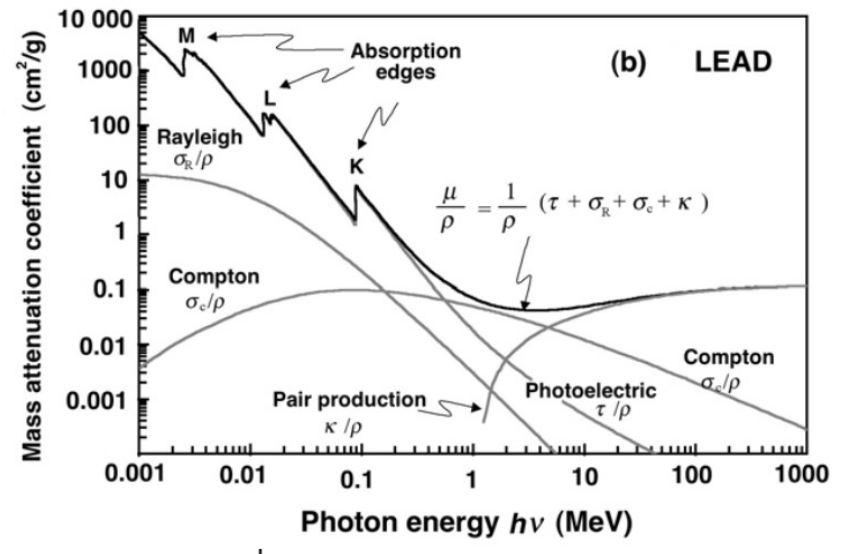
\includegraphics[width=0.5\linewidth]{Mass_Atenuacion.png}
    \end{figure}

    \textcolor{BrickRed}{Casi seguro es cierto.}
    \item Un valor aproximado de la eficiencia intrínseca para un fotopico a baja energía pdoría ser 70\% mientras que uno a alta energía 15\%. A bajas energías es casi seguro que va a depostiar toda su energía, mientras que a altas energías es probable que el fotón no deposite toda su energía. La eficiencia itnrínseca del detector a una energía determinada depende principalmente de si el fotón deposita toda su energía cinética en el detector o no, y esto depende del coeficiente de atenuación a dicha energía (que depende de la composición del detector),  del espesor y la geometría del detector. \textcolor{BrickRed}{Casi seguro es cierto.}
\end{enumerate}


\subsection{Montaje y prueba de un sistema para emdir la dispersión Compton}

\begin{enumerate}[label=\alph*)]
    \item Si la superficie es pequeña podemos aproximar elcálculo de la cantidad de gammas que llegan en el instante $t$ como:
    \begin{equation}
        N_{\text{llegan}} = \frac{\varepsilon_g A(t)B}{4\pi d^2}
    \end{equation}
    donde $\varepsilon_g$ es la eficiencia geométrica, $A(t)$ la actividad de la muestra en ese instnate, $B$ el braching ratio del canal $\gamma$ y $d$ la distancia.
    \item Teóricamente, la dispersión Compton es simétrica con respecto al eje de incidencia, ya que la ecuación de Compton y la sección eficaz de Klein–Nishina predicen que, para un fotón incidente, la distribución angular de los fotones dispersados es la misma a ambos lados del eje central. Sin embargo, en la práctica pueden aparecer pequeñas asimetrías debidas a factores geométricos, a la alineación del montaje y a la respuesta del detector. \textcolor{BrickRed}{Esta la pense yo, aunque chatgpt dijo algo parecido. Verificar.}
    \begin{itemize}
        \item Verificación de la simetría teórica: Al adquirir datos de ambos lados se puede confirmar que la distribución de la dispersión se ajusta a lo esperado según la teoría. Si se observan diferencias significativas, podría indicar problemas en el montaje o la necesidad de corregir efectos instrumentales.

        \item Corrección de efectos sistemáticos: Medir en ambos lados permite identificar y compensar posibles asimetrías del sistema experimental (por ejemplo, desalineaciones, diferencias en la eficiencia del detector o en el colimador) que podrían sesgar la medición de parámetros importantes como la sección eficaz de dispersión Compton.
    \end{itemize}
    \textcolor{BrickRed}{Verificar.}
    \item Debería estar balanecado. Lo ideal es encontrar un equilibrio: se debe elegir una distancia lo suficientemente grande para definir el ángulo de dispersión con precisión (minimizando la dispersión geométrica y asegurando que se cumple la aproximación puntual) pero sin que la reducción en la tasa de fotones comprometa la calidad estadística de la medición. La decisión final dependerá, entre otros factores, de la actividad de la fuente, de la sensibilidad del detector, de la eficiencia, geometría... \textcolor{BrickRed}{Yo pense exactamente lo mismo, debe estar bien.}
\end{enumerate}


\subsection{Medida de la relación energía-ángulo y de la sección eficaz de dispersión}

\begin{enumerate}[label=\alph*)]
    \item 
    Para calcular el número de centros dispersores (es decir, el número de electrones disponibles para interaccionar con la radiación gamma) en 1\,cm$^3$ de metacrilato, usamos la composición química del material. El metacrilato (PMMA) tiene como unidad repetitiva la fórmula:
    \[
    \mathrm{C_5H_8O_2}
    \]
    Esta fórmula indica que en cada unidad hay:
    \begin{itemize}
    \item 5 átomos de carbono: \(5 \times 6 = 30\) electrones  
    \item 8 átomos de hidrógeno: \(8 \times 1 = 8\) electrones  
    \item 2 átomos de oxígeno: \(2 \times 8 = 16\) electrones
    \end{itemize}
    En total, cada unidad contiene:
    \[
    30 + 8 + 16 = 54 \quad \text{electrones.}
    \]
    
    La masa molar aproximada de la unidad es:
    \[
    M \approx 5(12.01) + 8(1.008) + 2(16.00) \approx 60 + 8 + 32 \approx 100 \, \text{g/mol}.
    \]
    
    Si consideramos que la densidad del metacrilato es aproximadamente \(\rho = 1.18\, \text{g/cm}^3\), el número de moles en 1\,cm$^3$ es:
    \[
    n = \frac{\rho}{M} = \frac{1.18}{100} = 0.0118\, \text{mol/cm}^3.
    \]
    
    Multiplicando por el número de Avogadro (\(N_A \approx 6.022 \times 10^{23}\, \text{mol}^{-1}\)) obtenemos el número de moléculas por cm$^3$:
    \[
    N_{\text{moléculas}} = n \cdot N_A \approx 0.0118\, \text{mol/cm}^3 \times 6.022 \times 10^{23}\, \text{mol}^{-1} \approx 7.11 \times 10^{21}\, \text{moléculas/cm}^3.
    \]
    
    Dado que cada molécula tiene 54 electrones, el número total de electrones (centros dispersores) por cm$^3$ es:
    \[
    N_e = 7.11 \times 10^{21}\, \text{moléculas/cm}^3 \times 54 \approx 3.84 \times 10^{23}\, \text{electrones/cm}^3.
    \]
    
    Conociendo este valor, si se determina geométricamente el área del haz de radiación definido por el colimador y se conoce el espesor del bloque de metacrilato interceptado, se puede calcular el número total de centros dispersores en el volumen iluminado multiplicando \(N_e\) por el volumen efectivo (área por espesor). El número de centros dispersores efectivo vendrá dado por $N_{\text{dispersores}}=N_e \cdot A \cdot t$ donde $A$ es la superficie del haz y $t$ el grosor del metacrilato. \textcolor{BrickRed}{Creo que está bien hecho.}

    \item Al restar los espectros medidos con y sin el centro dispersor se obtiene un espectro “resta” que, en algunas regiones, puede presentar valores negativos en ciertos canales de energía. Esto se debe a las fluctuaciones estadísticas inherentes a la medición: cuando se sustrae un espectro de fondo de otro, las incertidumbres (que suelen ser de tipo Poisson, es decir, de la orden de la raíz cuadrada de los recuentos) pueden dar lugar a diferencias negativas en algunos bines, a pesar de que físicamente no se tengan “cuentas negativas”. Dicho de otra manera, estos valores negativos no indican una señal física negativa, sino que reflejan las variaciones aleatorias en los recuentos.

    En una región amplia en la que no se espera dispersión Compton del centro dispersor, el espectro resta debería tener un valor promedio cercano a cero. Esto es lo que se espera, ya que en esa región solo se cuenta con el fondo y sus fluctuaciones. En cuanto a los bines individuales, la dispersión alrededor de cero estará determinada por la incertidumbre estadística en cada canal, que es aproximadamente la raíz cuadrada de las cuentas medidas en ese bin. Por ejemplo, si en un canal el número de cuentas es de 100, la incertidumbre es de aproximadamente 10 cuentas, por lo que es normal observar valores en ese canal que fluctúan alrededor de cero en un rango de ±10 o ±20, dependiendo de la muestra y de las fluctuaciones aleatorias. \textcolor{BrickRed}{Tiene todo el sentido del mundo.}

    \item La pregunta se refiere a la determinación de la energía esperada del fotón dispersado en el espectro, es decir, en qué canal de energía del detector aparecerá un aumento en las cuentas debido a la dispersión Compton.

    Cuando un fotón gamma incide en el dispersor, puede sufrir una dispersión Compton, perdiendo parte de su energía y cambiando su dirección de propagación. El fotón dispersado tendrá una nueva energía $E$', que depende del ángulo de dispersión $\theta$ según la ecuación de Compton. Dado que los fotones dispersados llegarán al detector y formarán un exceso de cuentas en la región correspondiente a la energía $E$', el objetivo de la pregunta es determinar en qué canal de energía del espectro se debe observar este exceso para cada ángulo de dispersión. Para hacer un cálculo rápido se parte de la ecuación de Compton, que relaciona la energía \(E\)' del fotón dispersado con la energía inicial \(E\) y el ángulo de dispersión \(\theta\):
    \[
    E' = \frac{E}{1 + \frac{E}{m_e c^2}(1-\cos\theta)},
    \]
    donde \(m_e c^2 \approx 511\) keV. Por ejemplo, para una fuente de \(^{137}\)Cs con \(E=662\) keV y para \(\theta = 60^\circ\) (recordando que \(\cos 60^\circ = 0.5\)), se tiene:
    \[
    E' = \frac{662\,\text{keV}}{1 + \frac{662}{511}(1-0.5)} = \frac{662}{1 + \frac{662}{511}\times0.5}.
    \]
    Calculando, \(\frac{662}{511}\approx 1.30\) y \(\frac{662}{511}\times 0.5 \approx 0.65\); por lo que el denominador es \(1 + 0.65 = 1.65\) y, finalmente, 
    \[
    E' \approx \frac{662}{1.65}\approx 401\,\text{keV}.
    \]
    
    Este procedimiento se repite para cada ángulo: para cada valor central de \(\theta\) que determines en tu experimento, calculas \(E'\) y de esa forma sabes en qué canal de energía debería aparecer el exceso de cuentas debido a la dispersión Compton.
    
    Sin embargo, en la práctica, cuando se mide el espectro se observa que el exceso de cuentas se extiende sobre un rango de energía (una “dispersión” en energía) mayor que la simple energía calculada para un ángulo puntual. Esta dispersión en energía se debe a varios factores:
    \begin{itemize}
        \item Rango angular del sistema: Ni el detector ni el centro dispersor son puntos; el colimador define un haz con un ángulo de apertura \(\Delta \theta\). Dado que la relación \(E'(\theta)\) es no lineal, los fotones que inciden con ángulos dentro de \(\theta \pm \Delta \theta/2\) se dispersan con energías ligeramente distintas. Aproximadamente, la dispersión en energía se puede estimar como
           \[
           \Delta E \approx \left|\frac{dE'}{d\theta}\right|\Delta \theta.
             \]
         La derivada \(\frac{dE'}{d\theta}\) se evalúa en el ángulo central; de este modo, si el sistema tiene, por ejemplo, una apertura de 5° (convertida a radianes), la variación de energía será proporcional a este valor.
    
        \item Efectos geométricos: Además, la distribución espacial de la radiación y la extensión del dispersor y del detector implican que se recolectan fotones provenientes de un rango de posiciones y ángulos. Esto provoca que, en lugar de un pico estrecho, se observe un exceso de cuentas extendido en energía.
    \end{itemize}
    En resumen, para cada ángulo se calcula el \(E'\) esperado usando la ecuación de Compton. La dispersión observada en energía del exceso de cuentas se debe a que, en realidad, el sistema recoge fotones dispersados en un rango angular finito, lo que se traduce en una dispersión en la energía registrada. Esta dispersión puede, en gran medida, explicarse por la geometría del montaje, ya que ni el detector ni el centro dispersor son puntuales, sino que cubren una región angular determinada.

    \item  La sección eficaz aproximada se podrá obtener como:
    \begin{equation}
        \sigma = \frac{N_{det}}{N_e \Phi \Delta \Omega}
    \end{equation}
    donde $N_{det}$ son los fotones detectados para ese ángulo, $N_e$ el número de centros dispersores, $\Phi$ el flujo de electrones en el haz y $\Delta \Omega$ el ángulo sólido subtendido por el detector, que podremos comparar con la seección eficaz de Compton:
    \[
    \frac{d\sigma}{d\Omega} = \frac{r_0^2}{2} \left( \frac{E'}{E} \right)^2 \left( \frac{E}{E'} + \frac{E'}{E} - \sin^2\theta \right),
    \]
    
\end{enumerate}

\section{Medidas}

\subsection{Evaluación espectro 207Bi}

La primera media estuvo hecha a unos 6.2 + 0.8 cm cm (usando regla que mide milimetros, pegado a la caja gris). 

\subsection{Evaluación espectro 22Na}

La primera medida fue hecha a unos 6.2 cm (regla en milímetros).

\subsection{Evaluación espectro 60Co}

La primera medida fue hecha a 6.2 + 0.8 cm (regla en milímetros). 

\subsection{Evaluación del espector 152Eu}

La primera medida fue hecha a 6.2 +0.8 cm.

\subsection{Evaluación del espector 137Cs}

La primera medida fue hecha a 6.2 +0.8 cm.

\end{document}